\documentclass{beamer}
\usepackage[utf8]{inputenc}
\usepackage[T1]{fontenc}
\usepackage{graphicx}
\usepackage{tikz}
\usepackage{minted}
% \usepackage[texcoord,grid,gridunit=mm,gridcolor=red!20,subgridcolor=gray!10]{eso-pic}


\usemintedstyle{colorful}

\usetheme{avalon}
% \def\avalonprogressbar{1}
\def\avalondarkmintedstyle{zenburn}

\title{Avalon theme}
\subtitle{A modern theme for beamer}
\date{\it{}Somewhere in time \faMusic}
\author{Léo Valais}
\institute{Institute}

\titlegraphic{
  \vspace*{-1em}
  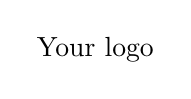
\begin{tikzpicture}
    \node () {Your logo};
  \end{tikzpicture}
}


\begin{document}

\begin{frame}
\titlepage
\end{frame}

\begin{frame}
  \frametitle{TOC}
  \tableofcontents{}
\end{frame}

\section{A theorem}
\begin{frame}
\frametitle{There Is No Largest Prime Number}
\framesubtitle{The proof uses \textit{reductio ad absurdum}.}
\begin{theorem}
There is no largest prime number. \end{theorem}
\begin{enumerate}
\item<1-| alert@1> Suppose $p$ were the largest prime number.
\item<2-> Let $q$ be the product of the first $p$ numbers.
\item<3-> Then $q+1$ is not divisible by any of them.
\item<1-> But $q + 1$ is greater than $1$, thus divisible by some prime
number not in the first $p$ numbers.
\end{enumerate}
\end{frame}

\section{Basic \LaTeX}
\subsection{Hmmm... some... items}
\begin{frame}{A longer title}
  \begin{itemize}
  \item one
  \item two
    \begin{itemize}
    \item two and half
    \item two and the.. other... half?
      \begin{itemize}
      \item no you don't
      \end{itemize}
    \end{itemize}
  \item \textrm{threee}
  \end{itemize}
\end{frame}

\subsection{Boxes}
\colorlet{mycolor}{iOS-red!25!white}
\begin{frame}{Thrid frame -- Amazing!}
  text

  \begin{tcolorbox}[frame hidden,fuzzy shadow={1mm}{-1mm}{0mm}{.3mm}{black},enhanced,colback=mycolor]
    big
  \end{tcolorbox}


  \begin{center}
    \tcbox[tcbox raise base,frame hidden,fuzzy
    shadow={.5mm}{-.5mm}{0mm}{.3mm}{black},enhanced,colback=mycolor]{small}
  \end{center}

  \begin{block}{blip}
    blop
  \end{block}
\end{frame}


\section{Awesome blueprint!}
\begin{blueprintframe}
  \frametitle{Blueprint}
\end{blueprintframe}

\section{Bye!}
\newcommand{\monly}[2]{\only<#1>{#2}}
\begin{frame}[fragile]
  \frametitle{The end.}
  Thx bye!
  \pause
  % dialog

  \pause
  Ya want sum code right?
  \pause
  % dialog

  \pause
  But ya want Lisp dont ya?
  \pause
  % dialog

  \pause
  \begin{block}[iOS-pink]{Now, for real}
    Goodbye!
  \end{block}

  \begin{popup}{0.75}
    \onslide<2>
    \begin{macosdialog}{Joking!}
      Itz \textbf{not} over yet!

      Aliquam erat volutpat. Nunc eleifend leo vitae magna. In id erat non
      orci commodo lobortis. Proin neque massa, cursus ut, gravida ut,
      lobortis eget, lacus. Sed diam. Praesent fermentum tempor tellus. Nullam
      tempus. Mauris ac felis vel velit tristique imperdiet. Donec at pede.
      Etiam vel neque nec dui dignissim bibendum. Vivamus id enim. Phasellus
      neque orci, porta a, aliquet quis, semper a, massa. Phasellus purus.
      Pellentesque tristique imperdiet tortor. Nam euismod tellus id erat.

      Aliquam erat volutpat. Nunc eleifend leo vitae magna. In id erat non
      orci commodo lobortis. Proin neque massa, cursus ut, gravida ut,
      lobortis eget, lacus. Sed diam. Praesent fermentum tempor tellus. Nullam
      tempus. Mauris ac felis vel velit tristique imperdiet.
    \end{macosdialog}

    \onslide<4>
    \begin{macosdarkdialog}{Here iz sum code for ya! :3}
      \begin{minted}[autogobble,breaklines,escapeinside=||]{latex}
\begin{popup}{0.75}
  \begin{macosdarkdialog}{Here iz sum code for ya! :3}
  \end{macosdarkdialog}
\end{popup}
      \end{minted}
    \end{macosdarkdialog}
  \end{popup}

  \begin{popup}{.75}
    \onslide<6>
    \begin{macosdarkdialog}{Slime REPL}
      \begin{minted}[autogobble,breaklines,escapeinside=||]{cl}
LISP> (setf a 12)
12
LISP> (if (zerop a) -1 a)
12
LISP> (defun fact (n)
        "Computes n!"
        (if (= n 0)
            1
            (* n (fact (1- n)))))
FACT
      \end{minted}
    \end{macosdarkdialog}
  \end{popup}
\end{frame}

\begin{frame}
  \nocite{*}
  \bibliographystyle{plain}
  \bibliography{example}
\end{frame}

\begin{standoutframe}
  \begin{center}
    \scalebox{1.5}[1.5]{\Huge \bfseries Any questions?}
  \end{center}
\end{standoutframe}

\begin{frame}[fragile]
  \frametitle{poij}
  \begin{alertblock}{Fuyez!}
    Pauvres fous...
  \end{alertblock}
  \begin{exampleblock}{Example}
\begin{minted}{ocaml}
let rec fact = function
  | 0 -> 1
  | x -> x * (fact (x - 1));;
\end{minted}
  \end{exampleblock}
  \begin{block}{Version using \texttt{if}}
 \begin{minted}{ocaml}
let rec fact x =
  if x = 0 then
    1
  else
    x * (fact (x - 1));;
\end{minted}
  \end{block}
\end{frame}
\end{document}
